\documentclass{article}
\usepackage[utf8]{inputenc}
\usepackage{graphicx}
\graphicspath{/home/tinob/study/intro\ ict}
\title{Assessment 1: My Profile}
\author{Tinotenda W. Bhebe}

\begin{document}
\rule{\linewidth}{1pt}

Name, Tinotenda Bhebe

Student ID: s3896133

GitHub PublicRepository URL:, 

GitHub Pages URL:

\maketitle
\tableofcontents
\section{Personal Information}

Tinotenda Wayne Bhebe:

born 18 feburary 2002 in Harare, Zimbabwe.

student id: s3896133

email: s3896133@student.rmit.edu.au

 educational history:

primary:
\begin{itemize}
   \item Midlands Christian School

    \item Horsham Primary School
    
    \item Sunshine Heights Primary

    \item Whitehorse Primary
  \end{itemize}
   
   secondary:
   \begin{itemize}
   
    \item Blackburn High School - High Achievers Program (HAP)
   
    \item officer secondary college 
    \end{itemize}
  
  languages spoken:
  \begin{itemize}
  
   \item Shona
  
   \item Ndebele
  
   \item English
\end{itemize}
  
  hobbies
  \begin{itemize}

   \item road bikes
  
   \item gym
  
   \item video games
  
   \item reading
  
   \item streaming content
\end{itemize}

\section{Interest in IT}


\subsection{What is your interest in it? }

my interest in information technology began at a very early age, my mother is a person who enjoys putting things together and this enjoyment has been passed on to me, i love putting electronics together and have strong thirst to understand how they work; in my latter years of high school i gained a strong interest in national security issues, from foreign relations to Cyber-warfare in 2018 mike burgess director general asd gave a speech to aspi whereby he said


 'Everything is being digitised, everything is being connected and everything is being controlled by software. And there is no doubt, the full potential of connectivity, technology and software are yet to be fully realised. However, these same benefits represent a significant risk.'


the quote at the time was the catalyst in my passion for for Cyber-security, i one day hope i can be there to mitigate the risks inherent in our modern world of interconnectivity; despite my passion for ict, i have very little experience working in the industry, what little experience i have comprises of working as a contractor to fix and refurbish old office computers as well as building/repairing personal computers and laptops. i hope to rectify this lack of experience in the coming years.
\newline

\subsection{why rmit?}

ict is a very complex and technical industry, when looking at job positions i quickly found that if i wanted to become a cybersecurity expert, i would require qualifications and experience, and with my lack of revenue i needed an educational institute that was relatively close to my home this critera made rmit an obvious choice, rmit is reputable for providing good quality education in stem and thus i chose to come to rmit and study the bachelor of information technology.\newline

\subsection{what do i expect to learn during my studies?}

upon finishing my studies i expect to have learnt the knowledge and expertise necessary to pursue my interests in cybersecurity and ict in general;
my skill set should be broad and adaptable to various environments since all workplaces are the same this includes skills in programming, networking and information security,
i also expect to have a broad knowledge base which forms an important foundation for further professional development, the ict industry is fast moving and workplaces will expect me to be able to
continuously learn new skills and techniques to more efficiently complete my job this includes a strong  working knowledge about cryptography, cloud systems, and programming; 
i don't expect to finish my course and be able to revolutionize the industry, instead i should have the skills and knowledge to pursue further education and work autonomously to complete organisational goals and objectives.

\section{Ideal Job}
\subsection{The job advertisement itself. Include a link, and a snapshot of it}
link: https://jobs.csiro.au/job/Canberra%2C-ACT-Cyber-Security-Operations-Manager/718989300/

\noindent snapshot: https://archive.is/hOWKe

\subsection{A description of the position, and its appeal}

the cyber security operations manager is a position where you lead cisros cybersecurity services, you job when simplified is the directing and leading csiros response to incidents and events, creation of new cyber attack tools and systems to improve responcse and minimise incidense
the job includes liasoning with law enforcemnt and government entities 

this jobs is appealing to me for various reasons, 
the role is a governemnt positions which allows me to work as a civil servant, there is a perceved job stability in being a civil servant in australian society, moreover it allows me to use my subject matter expertises to advance australian national interest and not just the interest of a company and its stakeholders;another facet of the jobs appeal is the leadership aspect of the role, the job allows me to be on the front line of australia cybersecurity policy an area of  personal interest to me, allowing me to not just work in cybersecurity, but to help and mentor employees in their duties and experiencies working for csiro cyber team.
\subsection{A description of the skills, qualifications and experience required for the position}

lots of theoreticl experience and practical experience in cybersecuirty for the role i would expect  a canadate to have a masters of cybersecurity or of a computing subject moreover i would also expect said canadate to have worked in the industry nto just in a cyber security team but also leading one, since csiro isnt just a workplace but australias principle science agency, a strong canadate would also require leadership skills beyond just managing a team but also, being accountable to stakeholders and being able to di
lastly a strong canadate for this role requires humility and academic thinking the cybersecuity field is quickly developing and requires quick contious personal development to keep up with the industry

\subsection{A description of the skills, qualifications and experience you have}
I currently only have my vce certificate as far as qualifications go; As a candidate for the cyber security team manager my vce certificate is not job relevant since the minimum expectation is tertiary education or 10years of industry experience.
I have the following workplace experiences:
4 years in the fast food industry which has allowed me to hone in the following workplace skills:
\begin{itemize}
\item interpersonal skills
\item teamwork skills
\item organization skills
\item stakeholder communication skills 
\end{itemize}
I also have experience in the youth organization Australian army cadets, this experience has helped me build great communication skills, leadership skills and accountability.  Whilst any workplace experience is better than none(cite) The position of cyber security team manager is a senior role whereby specialist experience and skills are required and all my skills experience and qualifications are below those required for entry level infotech jobs.

\subsection{A plan of how to obtain the skills for the position}

to one  day became a qualified canadate i should first complete my bachelors of it, i should then build upon it by getting in industry qualifications that will hopefully increase breadth of skills and my knowledge base this includes doing industry qualification such as ,Sans ccna, google it cert, aws,comptia security +,rhcsa, ccna, ocsp, gsec, gpen, dev ops engineer, cisco scyber, microsoft core, masterss
qualifications dont make up for a lack of live enironment experience
work in dev ops work in cybersec lead cybersec team work for thinktank  stregthen m aforementioned skills
beyond just qualifications i should also find work in the it industry most likely in cloud computing  etc etc etc 


\section{Personal Profile}
\subsection{Myers Briggs}
\begin{figure}[h]
\centering
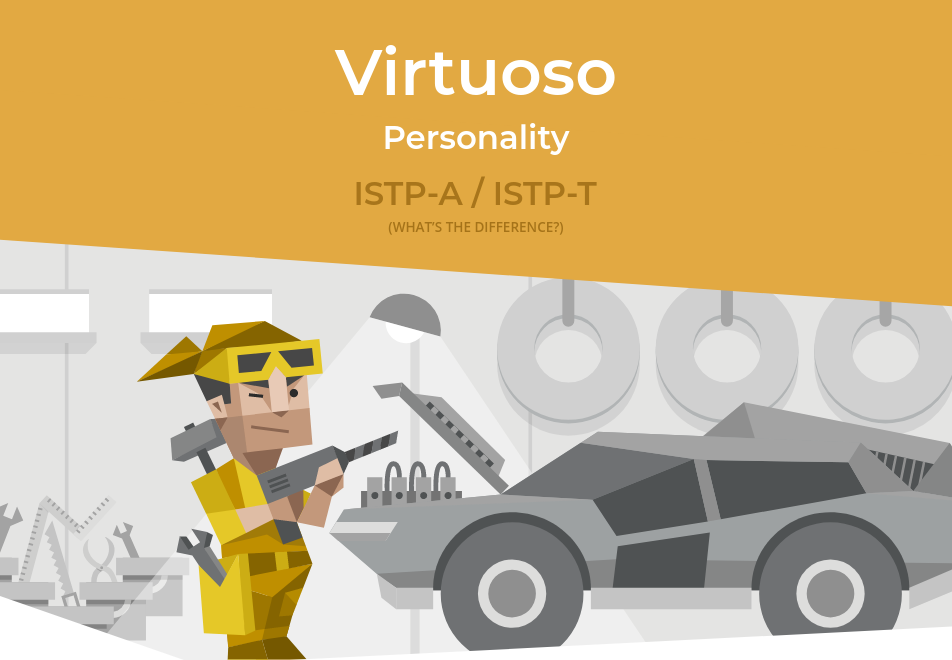
\includegraphics[width=\textwidth]{istp-t.png}
\caption{Myer briggs}
\end{figure}
 define myer briggs the vertuoso in a paragraph

 \subsection{EMTRAIN Learning Styles quiz}
\begin{figure}[h]
\centering
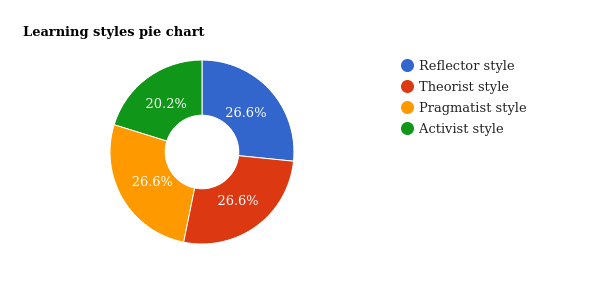
\includegraphics[width=\textwidth]{istp.png}
\caption{Myer briggs}
\end{figure}

\subsection{Hexaco}



\section{Project Idea}
\end{document}